

\section{Conception et développement de modèle}

Nous avons trouvé qu’il y a déjà beaucoup de projets sur la prédiction d’une séries temporelle financière. Pour atteindre notre objectif, nous avons proposé le modèle de réseaux neurones pour faire la prédiction. L’entrée et la sortie de notre projet sont très différentes par rapport aux autres projets. Les entrées sont les 13 TIs, comme nous savons plus de TIs peuvent apporter plus d’informations, mais il y a aussi plus de risques d’avoir trop de redondances. La sortie est le rendemnent sur un horizon prédefini, c’est plus difficile de prédire la vraie valeur que la tendance (mettre une seuil d’achat ou de vente). Dans cette partie, nous avons d'abord présenté la façon de construction de la base d'apprentissage, nous avons fait un pré-traitement sur les données origines et nous avons paramétré la base d'apprentissage. 

\subsection{Construction de la base d’apprentissage}

\subsubsection{Pré-traitement de données}

Comme nous avons pris un apprentissage supervisé, nous avons besoin d’abord d’ajouter les labels pour nos exemples, c’est-à-dire nous avons calculé le rendement sur un horizon pour chaque exemple. Le formulde de calculer le rendement est $ r = \frac{P_{t_{0}+h_{0}}}{P_{t_{0}}} - 1 $.

Dans un premier temps, nous avons utilisé directement les données non normalisées, parce que nous avions considéré que notre modèle peut ajuster les valeurs par lui-même, c'est-à-dire que la différence produit par l'échelle va être compensé automatiquement par les poids. Cependant, quand nous avons fait le premier test sur les données non normalisé, nous avons trouvé que le résultat n’était pas idéal. Le système n’a donné que un constant négatif et un constant positif comme le résultat, il n’a pas fait un rapprochement vers la vraie valeur. Ensuite, nous avons appliqué une normalisation aux entrées, nous avons pris le formulaire $(V-V_{min})/(V_{max}-V_{min})$, ça vaut dire que nous avons mis toutes les valeus de l’entrée sur la fourchette de [0,1]. Après la normalisation, nous pouvons trouver que le résultat était mieux et la valeur de prédiction a approché vers la vraie valeur.

\subsubsection{Paramétrage de la base d'apprentissage}

Pour notre projet, il faut aussi varier sur les paramètres différents pour construire la base d'apprentissage. Principalement, nous avons pris 4 indicateurs pour mesurer notre système, ils sont l'horizon, la taille d'apprentissage, la durée du test et le nombre de TI.

Pour lancer les simulations différentes, nous avons d'abord changé seulement un indicateur sur les tests différents. Et puis, nous pouvons tester sur le cas où nous pouvons changer 2 ou 3 indicateurs pour trouver le meilleur combinaison. 

Nous avons pris tous les 13 TIs au début de notre projet, nous voudrons collecter plus d’information pour faire la prédiction, nous avons considéré que cette combinaison de TI est plus robuste. Pour savoir le performance de notre système, nous avons diminué le nombre de TI, nous avons refait les tests avec la dimension réduite de TI. Pour l'instant, nous avons varié le nombre de TI sur 13, 12 et 4.

   	
\subsection{Choix du modèle}

Nous avons utilisé l'algorithme de perceptron multicouche à rétropropagation. Le perceptron multicouche est un type réseau organisé par plusieurs couches, chaque couche est constituée d'un nombre variable de neurones, les neurones de la dernière couche étant les sorties du système global. Dans notre cas, l'entré de reseau est les TIs et la sortie est le rendement. L'algoritnme de rétropropagation du gradient est pour minimiser l'erreur dans les systèmes multicouches. le figure \ref{fig:RN} pour représenter la structure de notre réseau neurone:

\begin{figure}
\centering
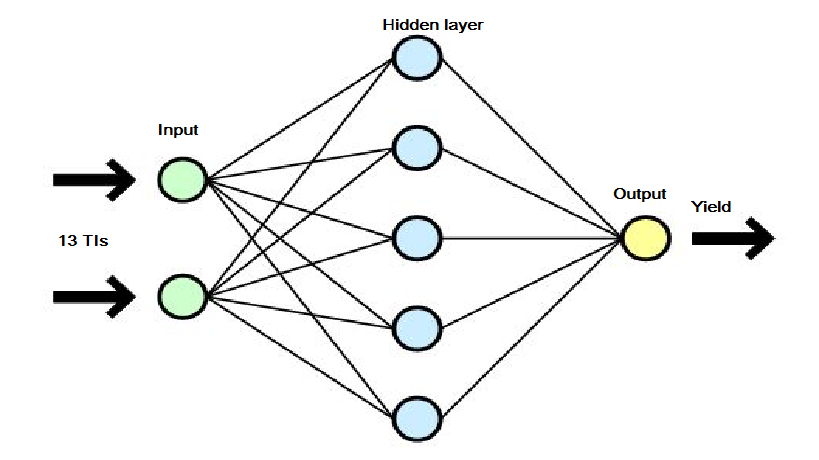
\includegraphics[width=.9\linewidth, scale=0.2]
{plot/RN.png}
\caption{Le schema de réseaux neurones}
\label{fig:RN}
\end{figure}

Pour être plus clair, nous avons présenté nos examples d'entrées en format matriciel : 

\begin{figure}
\centering
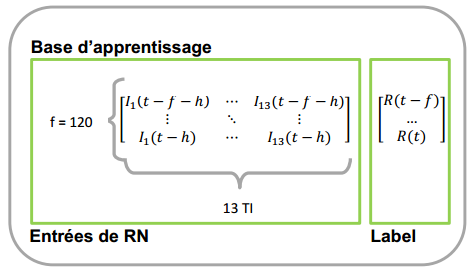
\includegraphics[width=.9\linewidth, scale=0.2]
{plot/base.png}
\caption{L'entrée de base d'apprentissage}
\label{fig:base}
\end{figure}




\subsection{Préparation des scénarios}